\chapter{Conclusion}
\epigraph{Of what a strange nature is knowledge! It clings to a mind when it has once seized on it like a lichen on a rock.}{Mary Shelley, \textit{Frankenstein; or, The Modern Prometheus}}


And thus, we have reached the end. In this thesis, we developed a general framework for improving the performance of model-based visual-inertial localization pipelines by complementing them with learned probabilistic ‘pseudo-sensors’ that extract difficult-to-model latent information from sensor data.  We presented four examples of such \textit{pseudo-sensors}.

\section{Summary of Contributions}

\noindent\textbf{Predictive Robust Estimation}

The contributions of PROBE are:
\begin{enumerate}
\item a probabilistic model for sparse stereo visual odometry, leading to a predictive robust algorithm for inference on that model,
\item a procedure for training our model using pairs of stereo images with known relative transform, and
\item an iterative, expectation-maximization approach to train our model when the relative ground truth egomotion is unavailable.
\end{enumerate}

\textbf{Publications}:

\begin{itemize}
	\item \bibentry{2016_Peretroukhin_PROBE-GK}
	\item \bibentry{2015_Peretroukhin_PROBE}
	\item \bibentry{2015_Peretroukhin_Get}
\end{itemize}

\noindent\textbf{Sun BCNN}

\begin{itemize}
	\item \bibentry{2018_Peretroukhin_Inferring}
	\item \bibentry{2017_Peretroukhin_Reducing}
	\item \bibentry{2017_Clement_Improving}
\end{itemize}

In Sun-BCNN, our main contributions can be summarized as follows:
\begin{enumerate}
\item We apply a Bayesian CNN to the problem of sun direction estimation, incorporating the resulting covariance estimates into a visual odometry pipeline; 
\item We demonstrate that a Bayesian CNN with dropout layers after each convolutional and fully-connected layer can achieve state-of-the-art accuracy at test time;
\item We learn a 3D unit-length sun direction vector, appropriate for full 6-DOF pose estimation;
\item We present experimental results on over 30~km of visual navigation data in urban \citep{Geiger2012-fq} and planetary analogue \citep{Furgale2012-kk} environments; 
\item We investigate the sensitivity of our Bayesian CNN-based sun estimator (Sun-BCNN) to cloud cover, camera and environment changes, and measurement parameterization; and
\item We release Sun-BCNN as open-source software\footnote{\url{https://github.com/utiasSTARS/sun-bcnn-vo}.}.
\end{enumerate}


\textbf{Deep Pose Corrections} \\
In summary, the main contributions of DPC:
\begin{enumerate}
	\item the formulation of a novel deep corrective approach to egomotion estimation,
	\item a novel cost function for deep $\LieGroupSE{3}$ regression that naturally balances translation and rotation errors, and
	\item an open-source implementation of DPC-Net in \texttt{PyTorch}\footnote{See \url{https://github.com/utiasSTARS/dpc-net}.}.
\end{enumerate}

\begin{itemize}
	\item \bibentry{2018_Peretroukhin_Deep}
\end{itemize}



\textbf{Estimating Rotation through Deep Probabilistic Inference with HydraNet} \\

The contributions of this work are:

\begin{enumerate}
\item a deep network structure we call \textit{HydraNet} that builds on prior work \cite{Lakshminarayanan2017,Osband2016} to produce meaningful uncertainties over unconstrained targets,
\item a loss formulation and mathematical framework that extends HydraNet to means and covariances of the rotation group $\LieGroupSO{3}$,
\item and open source code for $\LieGroupSO{3}$ regression\footnote{Repository redacted to protect author anonymity.}.
\end{enumerate}

\begin{itemize}
\item \bibentry{2019_Peretroukhin_Deep}
\end{itemize}


%\noindent\textbf{Other learning}
%
%\begin{itemize}
%	\item \bibentry{2017_Wagstaff_Improving}
%\end{itemize}

\section{Future Work}

\begin{figure}
\begin{center}
		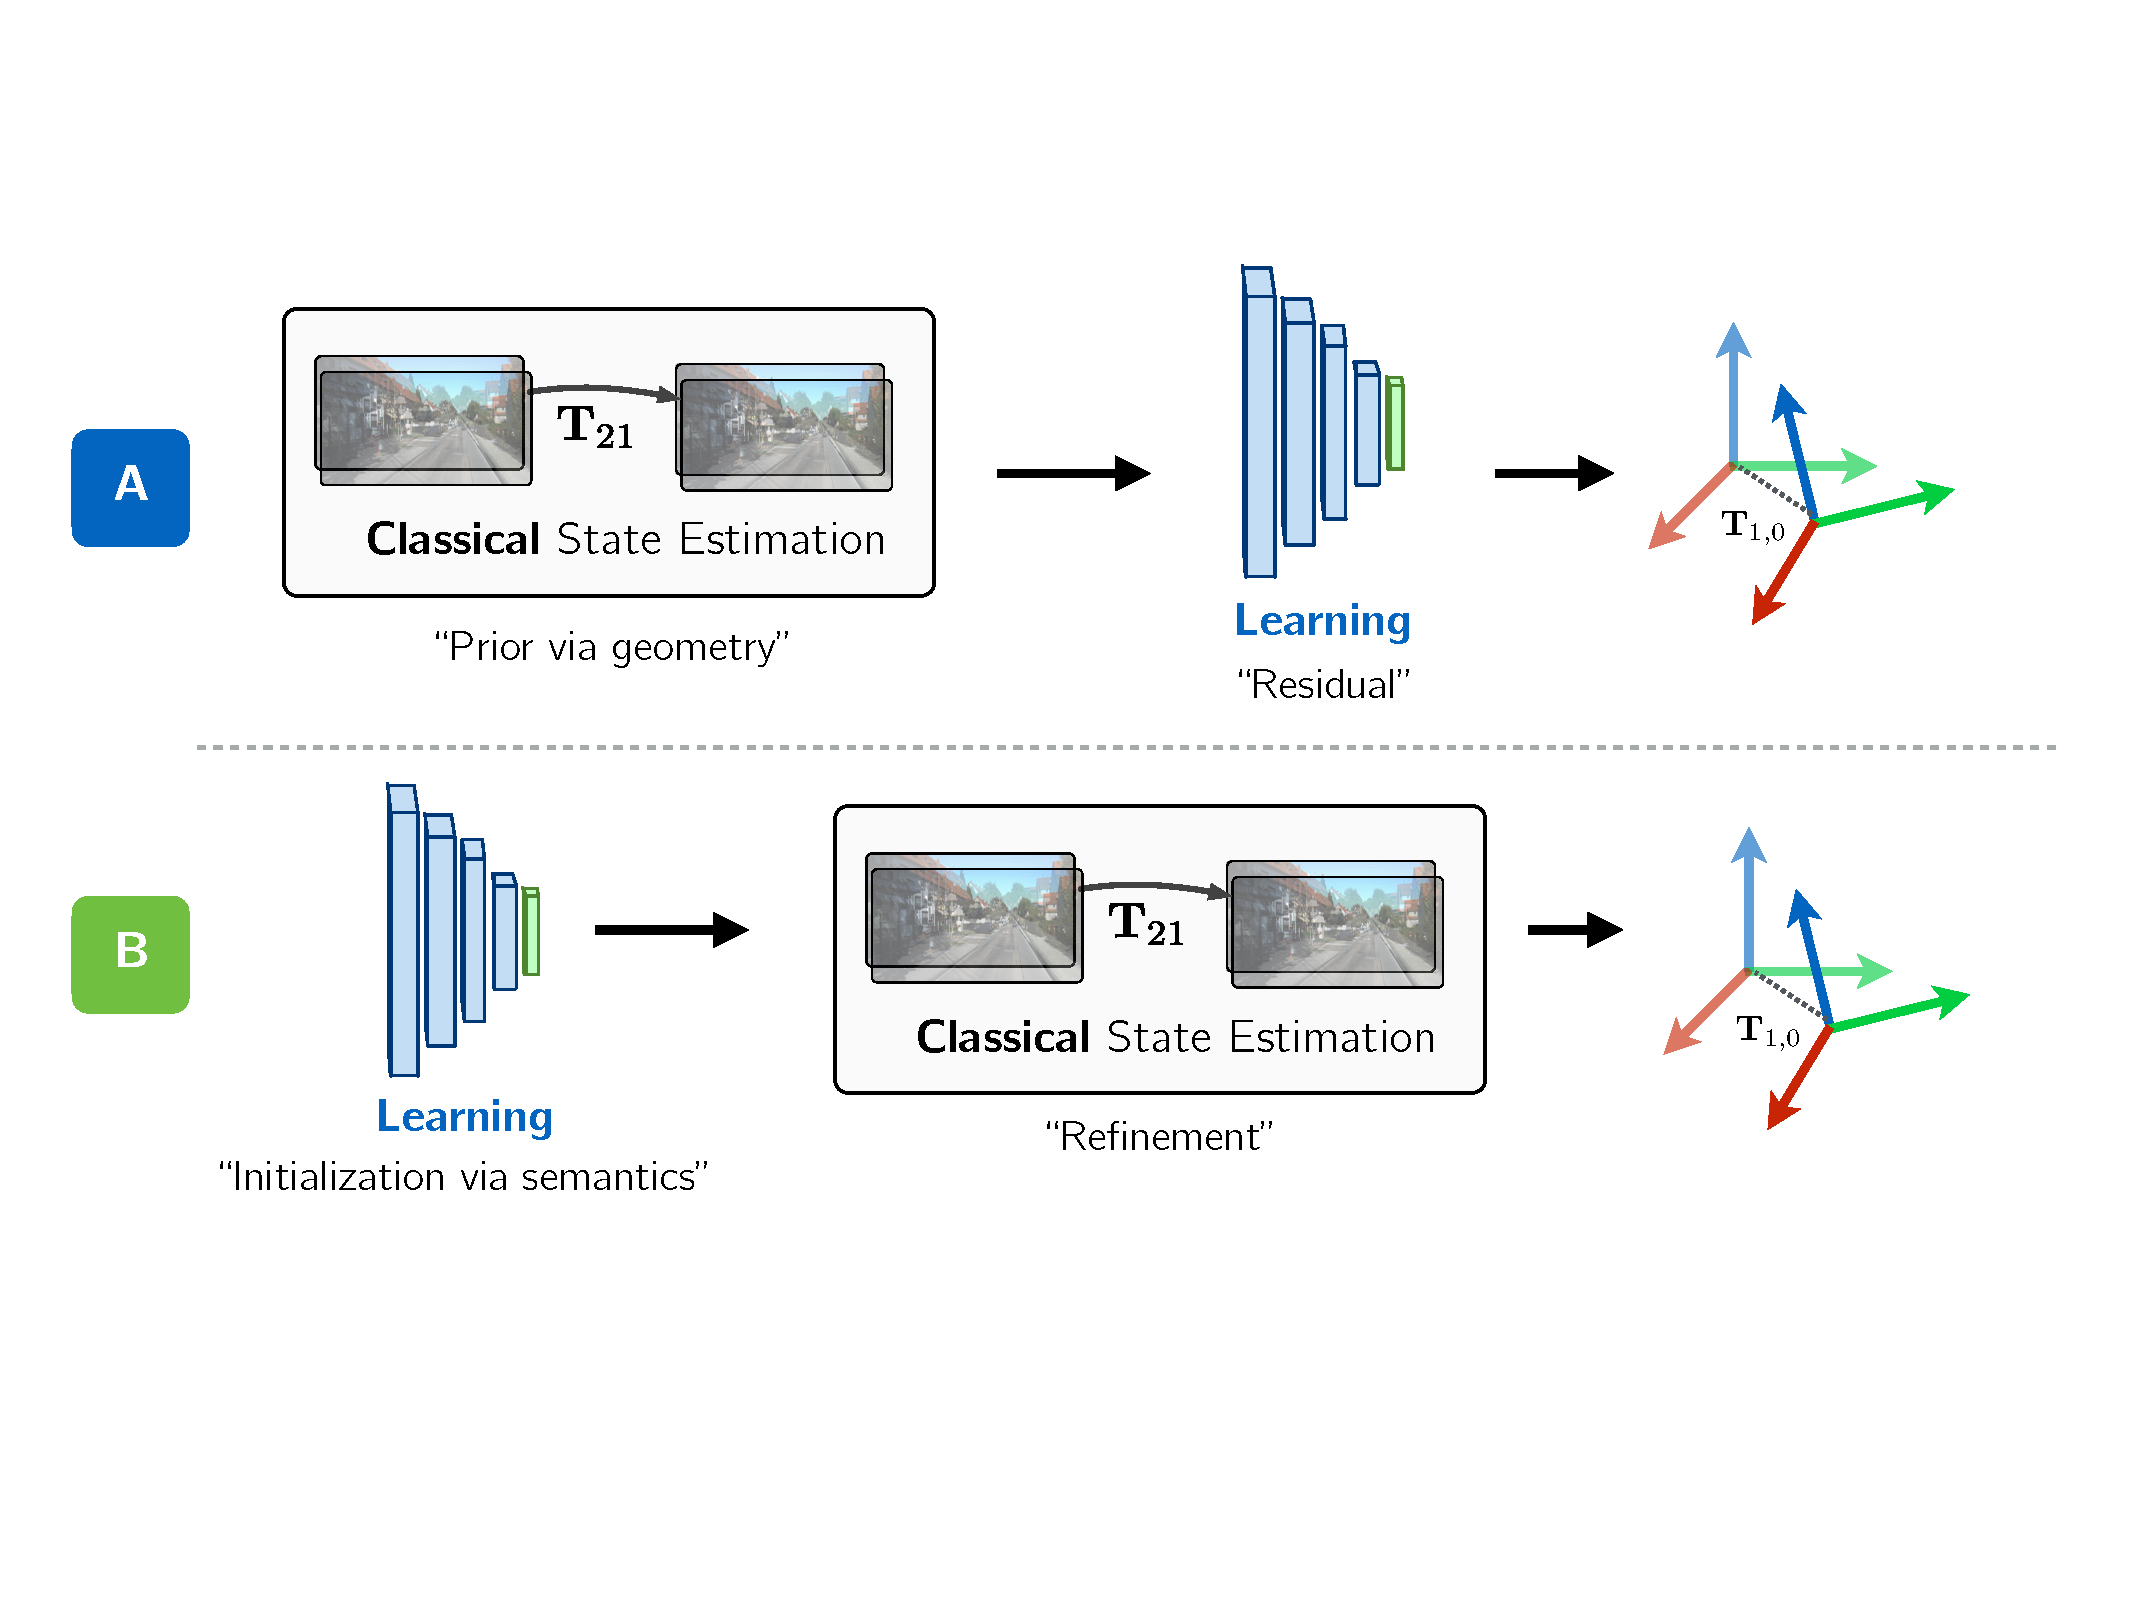
\includegraphics[width=0.98\textwidth]{conclusion/learning_as_prior.pdf}
		\caption{Two different ways to incorporate learning with classical pipelines. The first is by using pipelines as a \textit{prior} which can then be corrected by learned approaches, while the second is use learning as an initialization which can then be \textit{refined} by classical techniques.}
  	\label{fig:intro_vo_pipeline}
\end{center}
\end{figure}


There are many avenues for future work. For instance, although the fusion of pipelines with pseudo-sensors can significantly improve localization performance in a given environment, there are few guarantees that the final estimates are accurate and consistent

A potential thread of future work could address this deficiency by developing more tightly- coupled perception systems that can be ‘certified’ to produce globally-optimal solutions while still being robust to adverse environmental effects. By incorporating these learned ‘priors’ into an optimization framework, I plan to use recently- developed theory on convex relaxations (e.g., that presented in \todo{add citations here}) to ensure that the final localization and mapping results are ‘optimal’, in the sense that they are the global minima of a maximum-likelihood-based loss, and ‘safe’, in the sense that they provide consistent uncertainty estimates even in the presence of unmodelled effects. 

\section{Final Remarks}

The German Philosopher Georg Hegel had a particular dialectic method that involved a triad: a thesis, antithesis and synthesis.
Somewhat curiously, this \textit{thesis} has been an attempt at a \textit{synthesis} of the thesis posed by classical visual egomotion, and the antithesis posed by data-drive end-to-end learning techniques.
My hope is that the synthesis based on the concept of \textit{pseudo-sensors} will prove to be a fruitful one within the field of state-estimation, and for the broader robotics community.